% 
% sudo apt install texlive-fonts-extra
% may be requered sudo apt install cm-super
% 
% compile with pdflatex
%

\documentclass[hyperref={pdfpagelabels=false}]{beamer}
\usepackage{amssymb,cancel,cite,color,cmap,float,graphicx,lmodern,listings,
  multirow,pifont,pgfplots,txfonts,tikz,wrapfig,xcolor,yfonts}

\usepackage{paratype}
\renewcommand*\familydefault{\sfdefault}
\usepackage[T1, T2A]{fontenc}
\usepackage[utf8]{inputenc}
\usepackage[english,russian]{babel}

% some weird help from tex compiler
\pgfplotsset{compat=1.15}

\usetikzlibrary{arrows,automata,positioning,shapes,shapes.multipart}
\usetheme{Copenhagen}

\setbeamertemplate{navigation symbols}{}
%\addtobeamertemplate{number}{}{%
%    \usebeamerfont{footline}%
%    \usebeamercolor[black]{footline}%
%    \hspace{1em}%
%    \insertframenumber%/\inserttotalframenumber
%}

%\expandafter\def\expandafter\insertshorttitle\expandafter{%
%  \insertshorttitle\hfill%
%  \insertframenumber}
\newcommand*\circled[1]{\tikz[baseline=(char.base)]{
    \node[shape=circle,draw,inner sep=2pt] (char) {#1};}}
\addtobeamertemplate{navigation symbols}{}{
  \usebeamerfont{footline}
  \fontsize{14pt}{14}\selectfont
  \usebeamercolor[black]{footline}
  \hspace{1em}
  \circled{${\insertframenumber}$}
}
%\textswab
\setbeamertemplate{frametitle}[default][center]

\begin{document}
  
\title[Специализация алгоритма Витерби]{Специализация алгоритма Витерби на GPGPU скрытой марковской моделью}  
\author[И. Тюляндин]{Иван Тюляндин\\%
Научный руководитель: к.\,ф.-м.\,н., доцент С.\,В. Григорьев\\%
Консультант: к.\,ф.-м.\,н. Д.\,А.\,Березун\\%
} 
\date{9 июня 2020} 
{
\setbeamertemplate{navigation symbols}{}
\frame[noframenumbering,plain]{
\maketitle
} 
}


\begin{frame}{Предметная область(1)}
\begin{block}{Задача гомологичности}
	Поиск эволюционных предков у исследуемого протеина и изученных протеинов
	\begin{itemize}
		\item символьные последовательности
		\item вероятности сходства последовательностей
	\end{itemize}
\end{block}
\vfill
\begin{block}{Скрытые марковские модели и алгоритм Витерби}
\begin{itemize}
	\item профиль семейства через СММ
	\item алгоритм Витерби для проверки гомологичности
\end{itemize}
\end{block}
\end{frame} 


\begin{frame}{Предметная область(2)}
\begin{figure}
	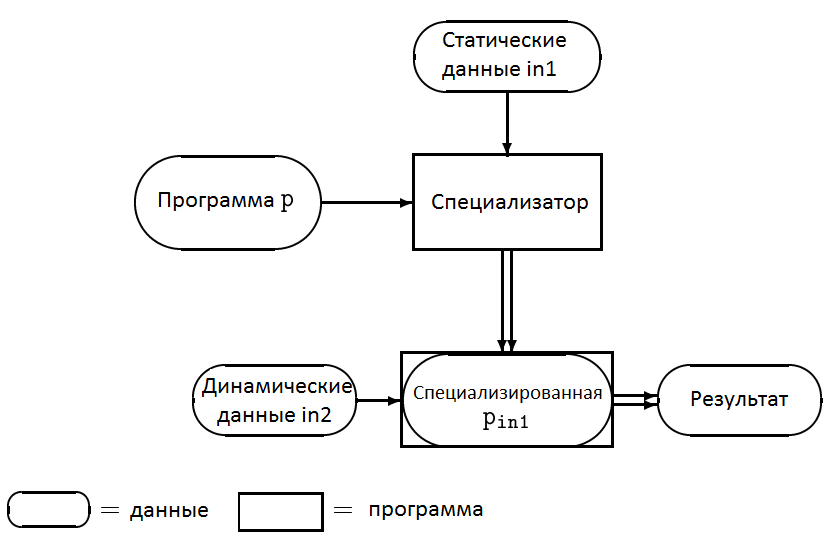
\includegraphics[scale=0.45]{spec.png}
	\caption{Специализация}
\end{figure}
\end{frame} 


\begin{frame}{Предметная область(3)}
\begin{block}{Специализация GPGPU}
	Идея: перенос статических данных в код уменьшит промахи кэша данных на 
	GPGPU
\end{block}
\vfill
Специализированный наивный поиск подстроки в строке быстрее в 8 раз
\end{frame} 

\begin{frame}{Цель}
\begin{block}{Цель}
Исследовать применимость специализации алгоритма Витерби, реализованного на 
GPGPU
\end{block}
\vfill
\begin{figure}
	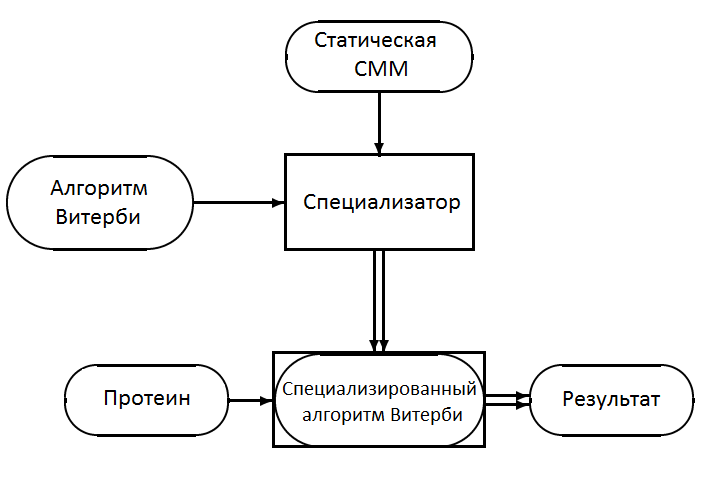
\includegraphics[scale=0.40]{spec_Viterbi.png}
\end{figure}
\end{frame}


\begin{frame}{Поставленные задачи}
\begin{itemize}
	\item Сделать обзор предметной области и существующих решений задачи 
		гомологичности
	\vfill
	\item Реализовать GPGPU версию алгоритма Витерби
	\vfill
	\item Написать специализатор алгоритма Витерби на СММ
	\vfill
	\item Провести сравнительный анализ производительности
\end{itemize}
\end{frame}


\begin{frame}{Текущие результаты}
\begin{itemize}
	\item Сделан обзор предметной области
	\begin{itemize}	
		\item задача гомологичности, СММ и алгоритм Витерби
		\item технологии программирования гетерогенных систем NVIDIA CUDA, 		
			OpenCL, SYCL
		\item техника специализации (в частности, для GPGPU кода)
		\item имеющиеся аналоги HMMer и CUDAMPF с вероятностным фильтром MSV
	\end{itemize}
	\vfill
	\item реализация алгоритмов для замеров
		\begin{itemize}
			\item чтение форматов fasta и hmm;
			\item однопоточная версия MSV алгоритма Витерби;
			\item многопоточная версия MSV дописывается;
		\end{itemize}
\end{itemize}
\vfill
Далее планируется перейти к написанию специализатора и проведению 
сравнительного анализа производительности.
\end{frame} 

\end{document}
